\appendix
\section{Demos}

We have constructed two demos that can serve the purpose of understanding the time synchronization and multi-hop data transmission in OpenWSN protocol. They are named \verb+demo_multihop_dict_nopower.xml+(see Figure~\ref{fig:multihop}) and \verb+demo_sync.xml+ in the accompanying folder with this report. Readers are welcome to open it and run it with Ptolemy II. 

\hide{
\begin{figure}[t]
\centering
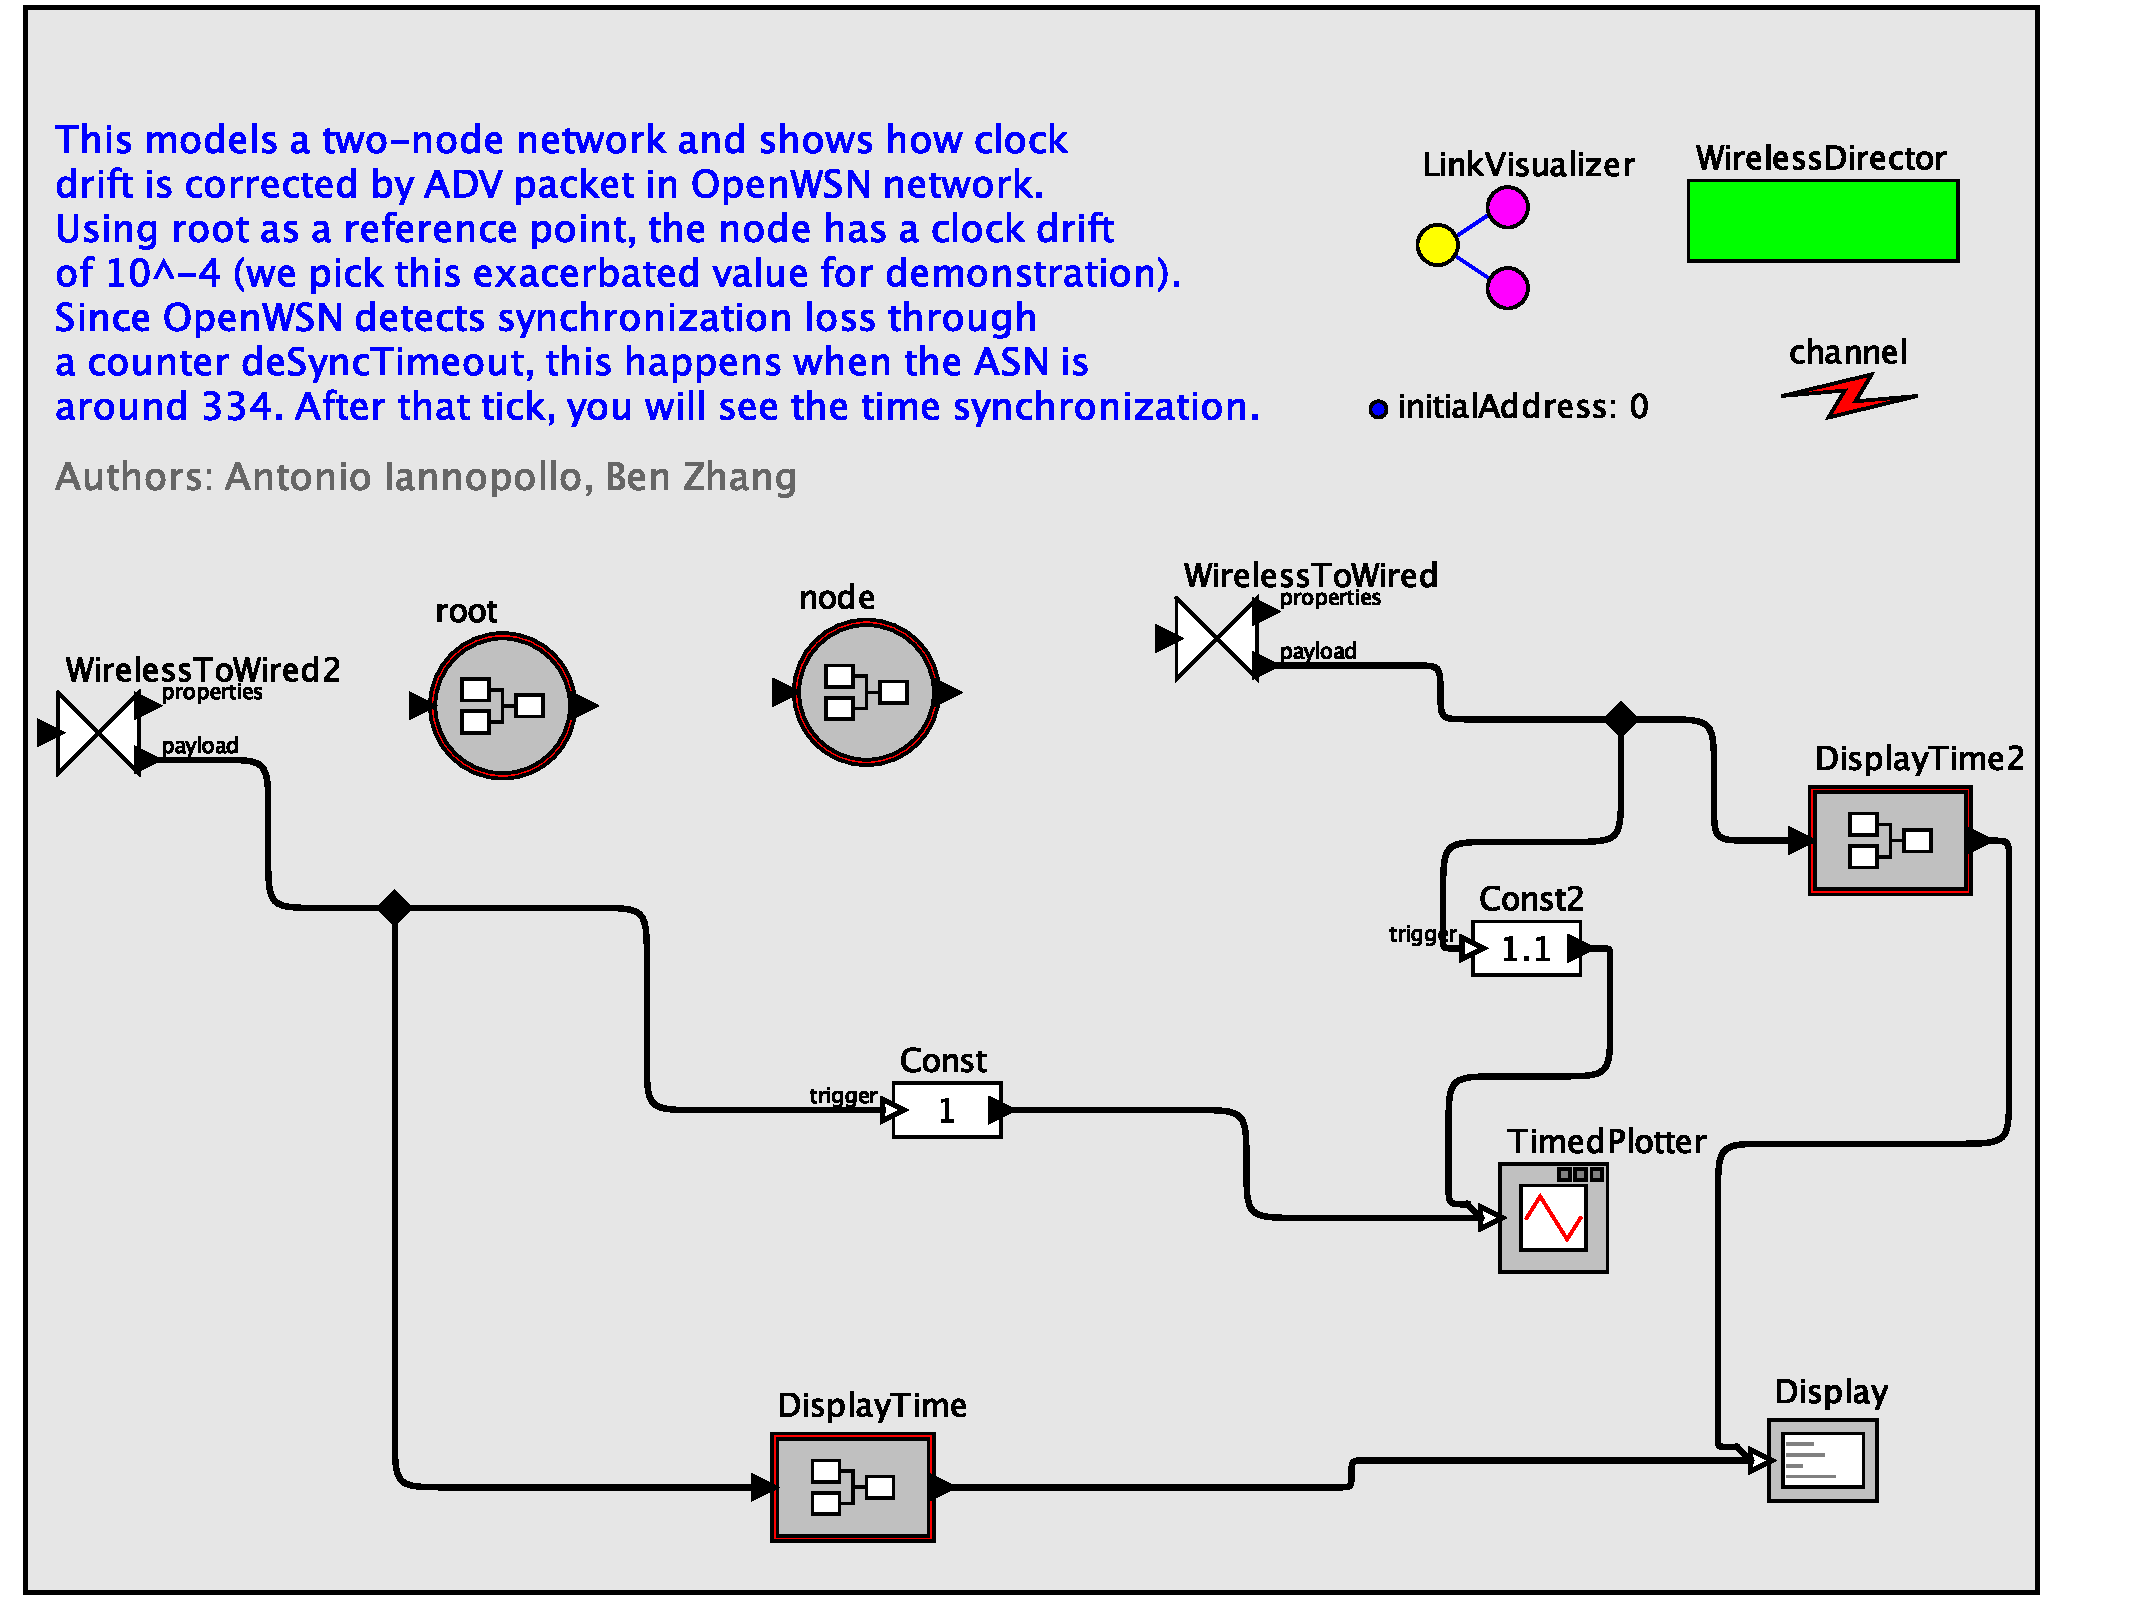
\includegraphics[width=0.7\columnwidth]{figures/PaperDemoSync}
\caption{\small Ptolemy demo that shows the action of time synchronization.}
\label{fig:timesync}
\end{figure}}


%%% Local Variables: 
%%% mode: latex
%%% TeX-master: "ee219d"
%%% End: 
